\subsection{\label{subsec:FZV4}Stokes Relation}
Die Stokes Relation stellt die Reflexions- und Transmissionskoeffizienten $r$ und $t$ anhand
eines zeitinvarianten Grenzflächenübergangs in Verbindung. Sie lässt sich anhand von Abb.~\ref{fig:stokes}
anschaulich herleiten.
\begin{figure}[h!]
  \centering
  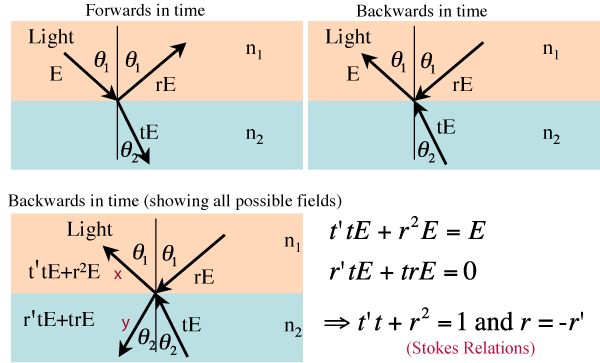
\includegraphics[width=0.4\textwidth]{Stokes.png}
  \caption{\label{fig:stokes}Skizze des Gedankenspiels zur Herleitung der Stokes Relationen.
    Der Reflexions- und Transmissionsprozess (obere Reihe) wird zeitlich umgekehrt und aufgrund von
    fehlender Absorption wird Invarianz vorausgesetzt. Aus der Zeitumkehr ergeben sich mögliche
    Felder (x und y), die mit dem ursprünglichen Prozess übereinstimmen müssen. Hieraus können die
    Stokes Relationen (unten rechts) abgeleitet werden. Die Grafik wurde Ref.~\cite{Stokes} entonommen.}
\end{figure}\FloatBarrier
Beim ursprünglich betrachteten Prozess (links oben) ist die reflektierte (transmittierte) Amplitude
des resultierenden Feldes durch $rE$ ($tE$) gegeben. Dreht man diesen Prozess um, so werden die
reflektierten und transmittierten Amplituden selbst als Eingangsfeld betrachtet, die an der
Grenzfläche wiederum Reflexion und Transmission erfahren. Übergänge innerhalb oder von Medium 2 (blau)
nach Medium 1 (orange) werden durch gestrichene Koeffizienten gekennzeichnet. Damit Zeitumkehrinvarianz
vorliegen kann, dürfen die Medien nicht absorbieren und müssen folglich als ideale Dielektrika vorliegen.
Der Brechungsindex ist daher eine rein reelle Größe ($\tilde{n} = n$).
Aus der Zeitumkehr kann man nun die Stokes Relationen herleiten, da die Situation links unten dem Ursprungssystem gleichen muss. \\
Mithilfe der Fresnelschen Formeln und dem Snelliusschen Brechungsgesetz können die Koeffizienten $r$ und $t$ in Abhängigkeit
der Winkel $\Theta_{1}$ und $\Theta_{2}$ dargestellt werden. Für TE-Wellen folgt
\begin{equation}
  t = \frac{2\sin(\Theta_{2})\sin(\Theta_{1})}{\sin(\Theta_{1} + \Theta_{2})}
  \hspace{1.5cm}
  r = -\frac{\sin(\Theta_{1} - \Theta_{2})}{\sin(\Theta_{1} + \Theta_{2})}.
\end{equation}
Bei der Zeitumkehr werden die Winkel andersherum definiert, was bedeutet, dass der Reflexionskoeffizient sein Vorzeichen dreht,
wohingegen die Transmission gleich bleibt.
Aus der ersten Stokes Relation kann man daher die Energieerhaltung erkennen
\begin{equation}
  t't + r^{2} = t^{2} + r^{2} = T + R = \frac{I_{\text{t}} + I_{\text{r}}}{I_{\text{i}}} = 1.
\end{equation}
Ist keine Absorption vorhanden, so muss sich die eingestrahlte Intensität auf die transmittierte und die reflektierte Intensität
verteilen. \\
Aus der zweiten Stokes Relation folgt, ein Phasensprung von $\pi$
bei der Reflexion an einem Medium, je nachdem von welcher Seite der Grenzfläche die Lichtwelle einfällt.
Hieraus lässt sich der Gangunterschied von $\lambda / 2$ aus Frage \ref{subsec:FZV2} erklären. \\
% [Eugene Hecht: Optics. 4th ed. Addison-Wesley, Reading, Mass. 2002, ISBN 0-8053-8566-5.
% Ariel Lipson, Stephen G. Lipson, Henry Lipson: Optical Physics. 4th ed. Cambridge University Press, Cambridge 2011, ISBN 978-0-521-49345-1.]